\documentclass{article}
\usepackage[utf8]{inputenc}

\title{Trabalho de Visão Relatório}
\author{Felipe Leivas Machado - 262528 \and Priscila Cavalli Rachevski - 261573 }
\date{September 2019}

\usepackage{natbib}
\usepackage{graphicx}

\begin{document}

\maketitle

\section{Questão 1}
    Nesta questão precisavamos desenhar uma linha para representar um jogador que estaria num certo ponto (X,Y), onde X e Y representam o pixel dos pés do jogador. Para podermos fazer isso precisavamos calcular algumas coisas, como:
   \begin{itemize}
       \item Gerar os pontos de calibragem
       \item Gerar a matriz P de calibragem da camera
       \item Converter uma cordenada 2D para uma cordenada 3D
       \item Converter uma cordenada 3D  para uma cordenada 2D
       \item Desenhar uma reta entre dois pontos
   \end{itemize}

    \subsection{Geração dos pontos}
        Para gerar os pontos pegamos alguns pontos fáceis de calcular a sua posição no mundo real. Os pontos selecionados estão destacados em vermelho, já o centro da imagem é o ponto azul:

        \begin{figure}[h!]
        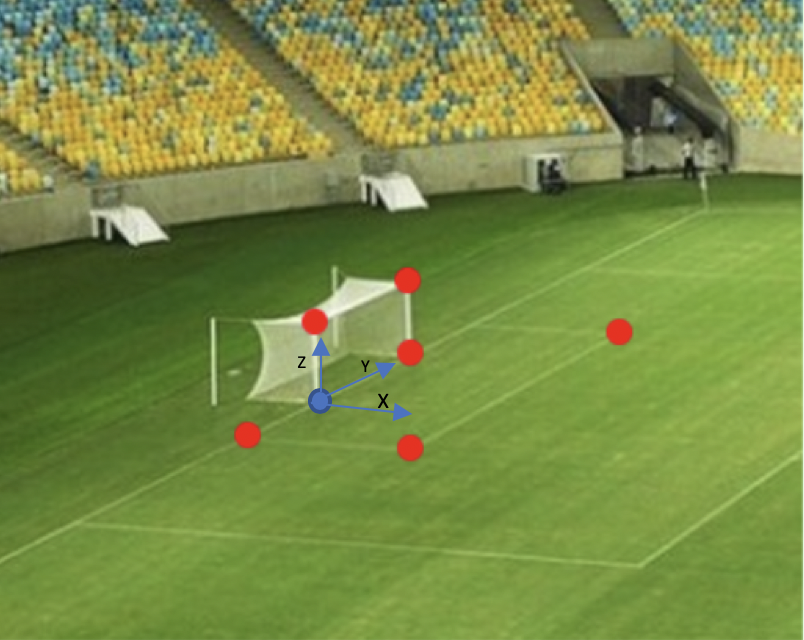
\includegraphics[scale=0.4]{maracana1Pontos.png}
        \end{figure}
    \subsection{Geração da Matriz de calibragem}
    Para geração da matriz de calibragem, primeiramente foi gerada a matriz A com base nos 6 pontos selecionados

\section{Conclusion}
``I always thought something was fundamentally wrong with the universe'' \citep{adams1995hitchhiker}

\bibliographystyle{plain}
\bibliography{references}
\end{document}
